% Provenance (never printed): old premiere S material on the structure of the
% Earth from seismology (P and S waves, travel times, the Moho, the shadow zone
% and the core, a reference model); see sources/book2/PROVENANCE.md. Profiles
% from figdata/grade-11/prem_profiles.py, rays and travel times from
% seismic_rays.py, the refraction lines and the problem's readings from
% moho_refraction.py. Lehmann's story and portrait are told in Book 1 (g6
% inside-the-earth): recalled here, not repeated.
\chapter{Las ondas sísmicas revelan el interior}\label{ch:g11:seismic-structure}

El 8 de octubre de 1909, un terremoto sacudió el valle del río Kupa, a unos
\qty{40}{km} al sureste de Zagreb, en Croacia. Unos meses antes, Andrija
Mohorovičić había instalado un sismógrafo nuevo en el Observatorio
Meteorológico de Zagreb, que registró todo el suceso. Después pidió sus
registros a otros observatorios y reunió los de 41 estaciones. En los
registros de las estaciones más lejanas encontró algo inesperado: dos \omterm{def:g11:seismic-structure:body-waves}{ondas P}
separadas, una débil y luego otra más fuerte, donde debería haber habido una
sola. De ese par de ondas dedujo que la roca situada bajo la corteza es
distinta, y midió la profundidad del límite. Este capítulo muestra cómo los
instantes en que llegan las ondas de los terremotos revelan las capas de la
Tierra: la base de la corteza, el núcleo y su parte externa líquida, y todo
el interior, profundidad a profundidad.
% ledger: herak:kupa-1909, srl:mohorovicic, geotech:moho-1909, kayal:pn-sn

\begin{recall}
Un terremoto empieza en un punto del interior de la Tierra, el hipocentro; el
punto de la superficie situado justo encima es el epicentro. Un sismómetro
registra las sacudidas del suelo, y la magnitud mide el tamaño de un
terremoto (Libro 1, año 7). La Tierra tiene una corteza, un manto y un
núcleo; el núcleo tiene una parte externa líquida y una parte interna sólida.
Las ondas de los terremotos son de dos tipos principales, las \omterm{def:g11:seismic-structure:body-waves}{ondas P}, más
rápidas, y las \omterm{def:g11:seismic-structure:body-waves}{ondas S}, más lentas, y las \omterm{def:g11:seismic-structure:body-waves}{ondas S} no pueden atravesar un
líquido (Libro 1, año 6). Una onda que atraviesa el límite entre dos
materiales en los que viaja a las velocidades $v_1$ y $v_2$ se refracta:
$\sin i_1/v_1 = \sin i_2/v_2$, donde los ángulos se miden respecto a la
perpendicular al límite (ley de Snell; los libros de física).
\end{recall}

\section{Las ondas sísmicas y los tiempos de recorrido}

\subsection{Dos tipos de ondas internas}

Un terremoto envía ondas en todas las direcciones. Unas viajan por la
superficie; otras, las ondas internas, viajan por el interior de la Tierra, y
son ellas las que lo revelan.

\begin{definition}[Onda P; onda S]\label{def:g11:seismic-structure:body-waves}
Una \emph{onda P}\index{onda P} es una onda sísmica que comprime y estira
alternativamente la roca: la roca se mueve hacia delante y hacia atrás en la
dirección en la que viaja la onda. Atraviesa sólidos, líquidos y gases, y es
la onda sísmica más rápida, así que llega la primera. Una \emph{onda
S}\index{onda S} cizalla la roca: la roca se mueve perpendicularmente a la
dirección en la que viaja la onda. Solo atraviesa sólidos, y llega después de
la onda P.
\end{definition}
% ledger: kayal:p-s

Un líquido fluye y no opone resistencia a un cambio de forma, así que no
puede transmitir una cizalla: por eso las \omterm{def:g11:seismic-structure:body-waves}{ondas S} se detienen en la
superficie de un líquido. En la mayoría de las rocas, una \omterm{def:g11:seismic-structure:body-waves}{onda P} viaja unas
$\sqrt 3 \approx 1.7$ veces más deprisa que una \omterm{def:g11:seismic-structure:body-waves}{onda S}.
En la corteza superior, una \omterm{def:g11:seismic-structure:body-waves}{onda P} viaja a unos \qty{5.8}{km/s} y una \omterm{def:g11:seismic-structure:body-waves}{onda S} a
unos \qty{3.2}{km/s}; justo debajo de la corteza alcanzan unos
\qty{8.1}{km/s} y \qty{4.5}{km/s}.
% ledger: kayal:p-s, kayal:outer-core-liquid, data:prem (vp_surface 5.8, vs_surface 3.2,
% vp_upper_mantle 8.11, vs_upper_mantle 4.49 in figdata/grade-11/prem_profiles.py)

\begin{omfigure}

\includegraphics[width=0.5\linewidth]{images/book2/g11-usgs-seismometer.jpg}

{\small Sismólogos de la Puerto Rico Seismic Network y del USGS instalan un
sismómetro temporal en el suroeste de Puerto Rico, el 10 de enero de 2020.
Fotografía: Thomas Pratt, USGS (dominio público).}
\end{omfigure}
% ledger: photo:g11-seismometer

\subsection{Las curvas de tiempos de recorrido}

La distancia de un terremoto a una estación lejana se mide como un ángulo: el
ángulo $\Delta$ en el centro de la Tierra entre el epicentro y la estación, la
\emph{distancia epicentral}\index{distancia epicentral}. Un grado de esta
distancia equivale a $\qty{111.2}{km}$ a lo largo de la superficie.
% ledger: earth:Rmean

\begin{definition}[Tiempo de recorrido; curva de tiempos de recorrido]\label{def:g11:seismic-structure:travel-time}
El \emph{tiempo de recorrido}\index{tiempo de recorrido} de una onda sísmica
en una estación es el tiempo que tarda en ir del hipocentro a la estación. La
\emph{curva de tiempos de recorrido}\index{curva de tiempos de recorrido} de
una onda es la gráfica de su tiempo de recorrido en función de la distancia
epicentral de la estación.
\end{definition}

Una estación registra el instante en que llega cada onda; cuando se conoce el
instante del terremoto, la diferencia es el \omterm{def:g11:seismic-structure:travel-time}{tiempo de recorrido}. Miles de
terremotos registrados por miles de estaciones han dado las \omterm{def:g11:seismic-structure:travel-time}{curvas de tiempos
de recorrido} con mucha precisión. En la figura, las curvas se han calculado
con el \omterm{def:g11:seismic-structure:reference-model}{modelo terrestre de referencia} de la \cref{sec:g11:seismic-structure:model},
y los puntos son \omterm{def:g11:seismic-structure:travel-time}{tiempos de recorrido} observados en terremotos reales: los dos
concuerdan en todas partes con un margen del dos por ciento, y casi siempre
con uno o dos segundos.

\begin{omfigure}
\begin{tikzpicture}
\begin{axis}[omrecord, width=0.84\linewidth, height=6.4cm, xmin=0, xmax=180, ymin=0, ymax=30,
  xtick={0,20,...,180}, ytick={0,5,...,30},
  xlabel={distancia epicentral $\Delta$ (grados)}, ylabel={tiempo de recorrido (minutos)},
  tick label style={font=\small}, label style={font=\small}, clip=false]
% computed in figdata/grade-11/seismic_rays.py; ledger: data:prem, auspass:surftim
\addplot[omDef, line width=0.9pt] table[x=delta_deg, y=t_min] {figdata/out/grade-11-seismic_rays-ttp.dat};
\addplot[omProp, line width=0.9pt] table[x=delta_deg, y=t_min] {figdata/out/grade-11-seismic_rays-tts.dat};
\addplot[omDef, line width=0.9pt, densely dashed] table[x=delta_deg, y=t_min] {figdata/out/grade-11-seismic_rays-ttpkp.dat};
\addplot[omDef!55, line width=0.9pt, densely dotted] table[x=delta_deg, y=t_min] {figdata/out/grade-11-seismic_rays-ttpkikp.dat};
\addplot[only marks, mark=*, mark size=1.5pt, black] table[x=delta_deg, y=p_min] {figdata/out/grade-11-seismic_rays-observed.dat};
\addplot[only marks, mark=*, mark size=1.5pt, black, unbounded coords=discard] table[x=delta_deg, y=s_min] {figdata/out/grade-11-seismic_rays-observed.dat};
\node[font=\small, text=omProp, anchor=south east] at (axis cs:68,21.2) {S};
\node[font=\small, text=omDef, anchor=north west] at (axis cs:72,11.2) {P};
\node[font=\small, text=omDef, anchor=south, align=center] at (axis cs:158,23.2) {P a través\\del núcleo};
\fill[black!10] (axis cs:98.5,0) rectangle (axis cs:143.8,3.2);
\node[font=\scriptsize, align=center] at (axis cs:121.1,1.6) {sin P directa};
\end{axis}
\end{tikzpicture}

{\small \omterm{def:g11:seismic-structure:travel-time}{Curvas de tiempos de recorrido} de las \omterm{def:g11:seismic-structure:body-waves}{ondas P} (azul) y de las \omterm{def:g11:seismic-structure:body-waves}{ondas S}
(naranja) de un terremoto en la superficie, calculadas con el \omterm{def:g11:seismic-structure:reference-model}{modelo
terrestre de referencia}; las curvas discontinua y punteada son \omterm{def:g11:seismic-structure:body-waves}{ondas P} que
han atravesado el núcleo (punteada: el núcleo interno). Puntos negros: \omterm{def:g11:seismic-structure:travel-time}{tiempos
de recorrido} observados. Entre unos \ang{99} y \ang{144} no llega
directamente ninguna \omterm{def:g11:seismic-structure:body-waves}{onda P} (zona sombreada).}
\end{omfigure}

La curva S sube con más pendiente que la curva P, así que el retraso entre
las dos llegadas crece con la distancia. Esto da la distancia de un terremoto
a partir de un solo registro.

\begin{method}[Distancia de un terremoto a partir del retraso S--P]\label{met:g11:seismic-structure:distance}
\begin{enumerate}
  \item En el registro, lee el instante de la primera \omterm{def:g11:seismic-structure:body-waves}{onda P} y el de la
        primera \omterm{def:g11:seismic-structure:body-waves}{onda S}; su diferencia es el retraso S--P.
  \item En las \omterm{def:g11:seismic-structure:travel-time}{curvas de tiempos de recorrido} (o en una tabla de ellas),
        busca la distancia epicentral a la que la curva S está ese retraso
        por encima de la curva P.
  \item Si hace falta, conviértela a kilómetros con $\qty{111.2}{km}$ por
        grado.
\end{enumerate}
Con tres estaciones, el epicentro es el punto que está a la distancia
correcta de las tres.
\end{method}

\begin{example}[Un terremoto a \ang{60}]\label{ex:g11:seismic-structure:sp}
Los \omterm{def:g11:seismic-structure:travel-time}{tiempos de recorrido} observados son de \qty{608}{s} para la P y
\qty{1101}{s} para la S a \ang{60}, y de \qty{536}{s} y \qty{967}{s} a
\ang{50}. Una estación que registra una \omterm{def:g11:seismic-structure:body-waves}{onda S} \qty{493}{s}
(8~minutos 13~segundos) después de la \omterm{def:g11:seismic-structure:body-waves}{onda P} está, por tanto, a \ang{60} del
epicentro: unos $60 \times 111.2 \approx
\qty{6670}{km}$. A \ang{50}, el retraso solo sería de \qty{431}{s}.
\end{example}
% ledger: auspass:surftim

\begin{omfigure}
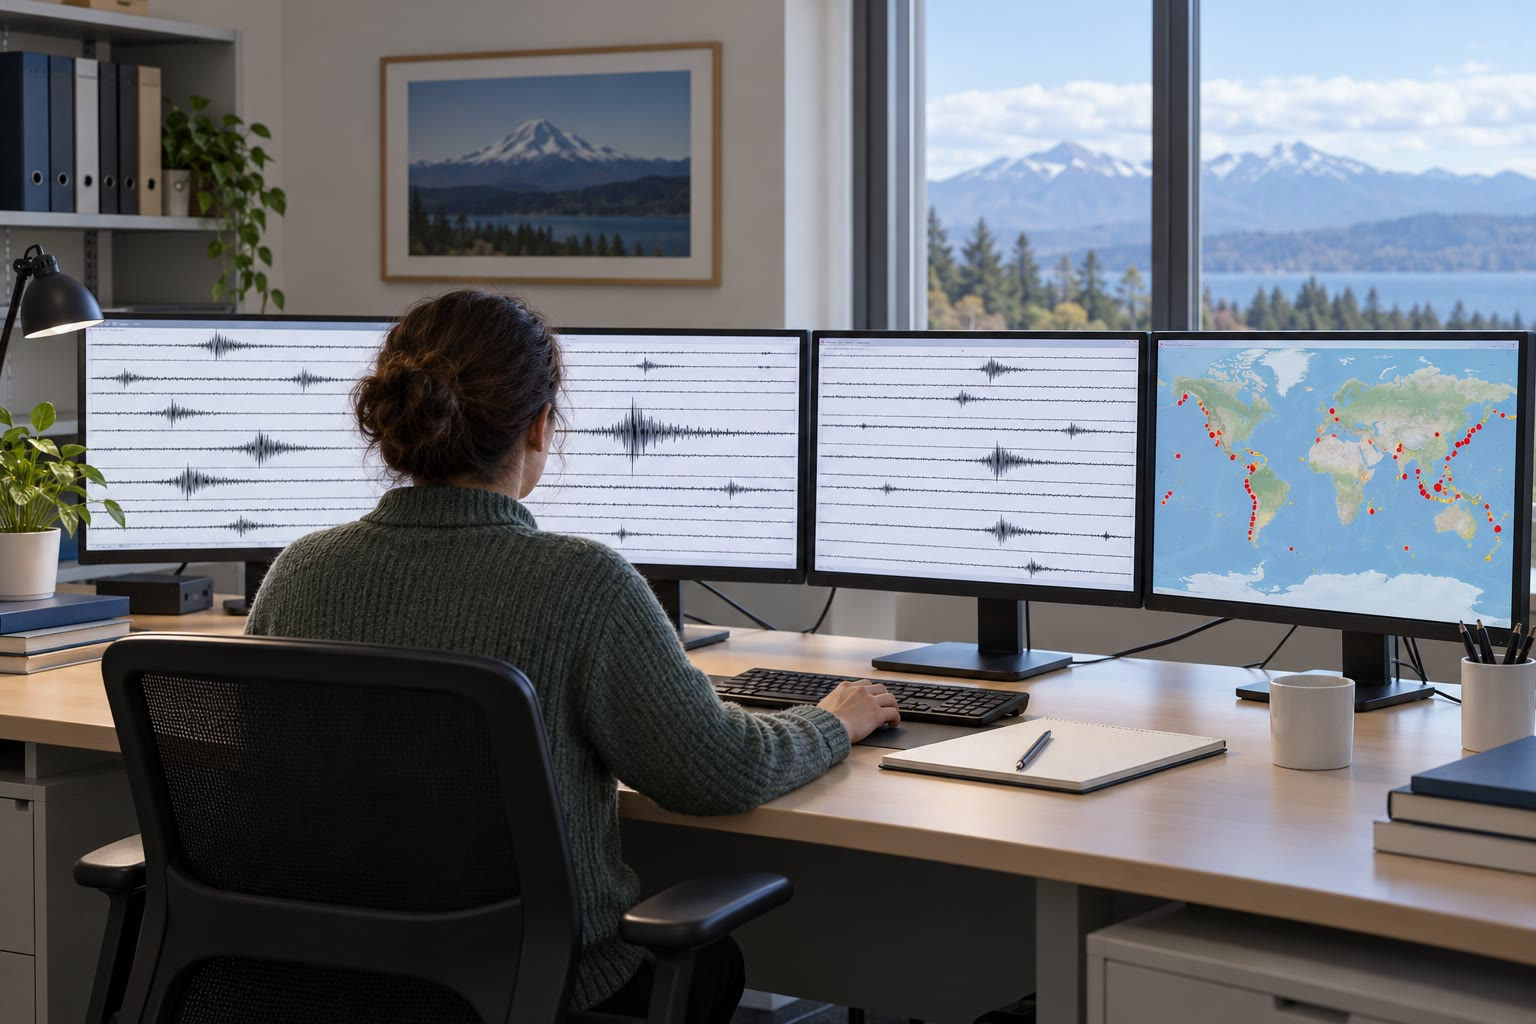
\includegraphics[width=0.66\linewidth]{images/book2/ai/g11-seismology-observatory.jpg}

{\small En un observatorio sismológico, los registros de muchas estaciones se
muestran uno junto a otro, y los terremotos que localizan se sitúan en un
mapa del mundo (ilustración generada por IA).}
\end{omfigure}

\section{La refracción y el Moho}\label{sec:g11:seismic-structure:moho}

\subsection{La onda que corre a lo largo de un límite}

En el interior de la Tierra, la velocidad de las ondas sísmicas cambia con la
profundidad, casi siempre de forma gradual, pero en algunos lugares de golpe.

\begin{definition}[Discontinuidad sísmica]\label{def:g11:seismic-structure:discontinuity}
Una \emph{discontinuidad sísmica}\index{discontinuidad sismica@discontinuidad sísmica}
es una superficie del interior de la Tierra a través de la cual la velocidad
de las ondas sísmicas cambia bruscamente --- en un espesor mucho menor que la
longitud de las ondas.
\end{definition}

En una discontinuidad, parte de la onda se refleja y parte se refracta. Tomemos
una capa de espesor $h$ en la que las \omterm{def:g11:seismic-structure:body-waves}{ondas P} viajan a $v_1$, sobre una capa
en la que son más rápidas, $v_2 > v_1$. Un rayo que baja con el ángulo $i$
respecto a la vertical se refracta con el ángulo $r$ dado por $\sin r = (v_2/v_1)\sin
i$: se aparta de la vertical. Cuando $\sin i$ llega a $v_1/v_2$, el
rayo refractado corre exactamente a lo largo del límite. El ángulo
\[
  i_c, \qquad \sin i_c = \frac{v_1}{v_2},
\]
es el \emph{ángulo crítico}\index{angulo critico@ángulo crítico}. La onda
refractada con el \omterm{ex:g11:seismic-structure:sp}{ángulo crítico} viaja por la parte alta de la capa más
rápida a la velocidad $v_2$ y, a medida que avanza, devuelve ondas hacia
arriba, a la capa superior, todas con el ángulo
$i_c$: llegan a la superficie como la \emph{onda de cabeza}\index{onda de cabeza}.

\begin{omfigure}
\begin{tikzpicture}[x=0.05cm, y=0.05cm, font=\footnotesize, >={Stealth[length=4pt]}]
% geometry from figdata/grade-11/moho_refraction.py: v1 6.2, v2 8.1, h 30 km, ic 49.9 deg
  \fill[omLithGranite!45] (-10,0) rectangle (215,-30);
  \fill[omLithPeridotite!45] (-10,-30) rectangle (215,-48);
  \draw[line width=0.6pt] (-10,0) -- (215,0);
  \draw[line width=0.9pt] (-10,-30) -- (215,-30);
  \node[anchor=west, align=left] at (218,-15) {corteza\\$v_1 = \qty{6.2}{km/s}$};
  \node[anchor=west, align=left] at (218,-39) {manto\\$v_2 = \qty{8.1}{km/s}$};
  \node[anchor=east] at (215,-26) {Moho};
  % source and station
  \fill[omDef] (0,0) circle (1.6);
  \node[anchor=south] at (0,1.5) {terremoto};
  \draw[fill=white] (197,0) -- (203,0) -- (200,5) -- cycle;
  \node[anchor=south] at (200,5) {estación};
  % direct wave
  \draw[->, omProp, line width=0.8pt] (2,-2) -- (196,-2);
  \node[anchor=south, text=omProp] at (100,0.3) {onda directa, velocidad $v_1$};
  % head wave
  \draw[omDef, line width=0.9pt] (0,0) -- (35.7,-30);
  \draw[->, omDef, line width=0.9pt] (35.7,-30) -- (100,-30);
  \draw[omDef, line width=0.9pt] (100,-30) -- (164.3,-30) -- (200,0);
  \node[anchor=north, text=omDef] at (100,-31) {a lo largo del Moho a $v_2$};
  \foreach \x in {50,70,90,110,130,150} {
    \draw[->, omDef!60, densely dashed] (\x,-30) -- ++(25.5,21.5);
  }
  % critical angle
  \draw[black!60, densely dotted] (35.7,-30) -- (35.7,-8);
  \draw[black!70] (35.7,-18) arc[start angle=90, end angle=130.05, radius=12];
  \node[anchor=south east] at (33,-16) {$i_c$};
  % thickness and critical distance
  \draw[<->] (-6,0) -- (-6,-30);
  \node[anchor=east] at (-7,-15) {$h$};
\end{tikzpicture}

{\small La onda directa y la \omterm{ex:g11:seismic-structure:sp}{onda de cabeza} (a escala: corteza de
\qty{30}{km} de espesor). La \omterm{ex:g11:seismic-structure:sp}{onda de cabeza} baja con el \omterm{ex:g11:seismic-structure:sp}{ángulo crítico} $i_c$,
corre por la parte alta del manto y vuelve a subir con $i_c$; a lo largo de
todo su recorrido por el \omterm{def:g11:seismic-structure:moho}{Moho} envía ondas hacia la superficie (discontinuas).
No llega a ninguna estación situada a menos de $2h\tan i_c$, unos
\qty{71}{km} aquí.}
\end{omfigure}

\begin{proposition}[Tiempo de recorrido de la onda de cabeza]\label{prop:g11:seismic-structure:head-wave}
Para una fuente en la superficie, una estación situada a la distancia
$x \ge 2h\tan i_c$ recibe la \omterm{ex:g11:seismic-structure:sp}{onda de cabeza} al cabo de
\[
  t(x) = \frac{x}{v_2} + \frac{2h\cos i_c}{v_1}.
\]
Su \omterm{def:g11:seismic-structure:travel-time}{curva de tiempos de recorrido} es una recta de pendiente $1/v_2$ que,
prolongada hacia atrás, corta el eje de tiempos en el \emph{tiempo de
intercepción}\index{tiempo de intercepcion@tiempo de intercepción}
$t_i = 2h\cos i_c/v_1$.
\end{proposition}

\begin{proof}
El rayo baja por un tramo inclinado de longitud $h/\cos i_c$, que avanza
horizontalmente $h\tan i_c$; hace lo mismo al subir. Entre medias corre
a lo largo del límite una distancia $x - 2h\tan i_c$. El tiempo es
\[
  t = \frac{2h}{v_1\cos i_c} + \frac{x - 2h\tan i_c}{v_2}
    = \frac{x}{v_2} + \frac{2h}{v_1\cos i_c} - \frac{2h\sin i_c}{v_2\cos i_c}.
\]
Como $1/v_2 = \sin i_c/v_1$, los dos últimos términos dan
$\frac{2h}{v_1\cos i_c}\,(1 - \sin^2 i_c) = \frac{2h\cos i_c}{v_1}$.
\end{proof}

La onda directa llega al cabo de $x/v_1$: su curva es una recta que pasa por
el origen, con más pendiente que la recta de la \omterm{ex:g11:seismic-structure:sp}{onda de cabeza}. Cerca de la
fuente llega primero la onda directa; lejos, la \omterm{ex:g11:seismic-structure:sp}{onda de cabeza}, que ha hecho
la mayor parte del camino a la velocidad más alta, la adelanta.

\begin{proposition}[Distancia de cruce]\label{prop:g11:seismic-structure:crossover}
La \omterm{ex:g11:seismic-structure:sp}{onda de cabeza} llega antes que la onda directa más allá de la
\emph{distancia de cruce}\index{distancia de cruce}
\[
  x_c = 2h\sqrt{\frac{v_2 + v_1}{v_2 - v_1}}.
\]
\end{proposition}

\begin{proof}
Las dos ondas llegan a la vez cuando $x/v_1 = x/v_2 + 2h\cos i_c/v_1$, es decir,
$x\,(v_2 - v_1)/(v_1 v_2) = 2h\cos i_c/v_1$, luego $x = 2h\cos i_c\,v_2/(v_2 -
v_1)$. Ahora bien, $\cos i_c = \sqrt{1 - v_1^2/v_2^2} = \sqrt{(v_2 - v_1)(v_2 +
v_1)}/v_2$, de donde $x = 2h\sqrt{(v_2 + v_1)(v_2 - v_1)}/(v_2 - v_1) =
2h\sqrt{(v_2 + v_1)/(v_2 - v_1)}$. Más allá, la \omterm{ex:g11:seismic-structure:sp}{onda de cabeza}, cuya recta
tiene menos pendiente, llega primero.
\end{proof}

\begin{omfigure}
\begin{tikzpicture}
\begin{axis}[omrecord, width=0.78\linewidth, height=5.6cm, xmin=0, xmax=300, ymin=0, ymax=50,
  xtick={0,50,...,300}, xlabel={distancia al epicentro (\unit{km})}, ylabel={tiempo de recorrido (\unit{s})},
  tick label style={font=\small}, label style={font=\small}, clip=false]
% computed in figdata/grade-11/moho_refraction.py (critical_km 71.4, crossover_km 164.6, intercept_s 6.23)
\addplot[omProp, line width=0.9pt] table[x=x, y=tdirect] {figdata/out/grade-11-moho_refraction-model.dat};
\addplot[omDef, line width=0.9pt, restrict x to domain=71:300] table[x=x, y=thead] {figdata/out/grade-11-moho_refraction-model.dat};
\addplot[omDef, densely dashed, restrict x to domain=0:72] table[x=x, y=thead] {figdata/out/grade-11-moho_refraction-model.dat};
\draw[black!50, densely dotted] (axis cs:164.6,0) -- (axis cs:164.6,26.5);
\node[font=\scriptsize, anchor=north] at (axis cs:164.6,0) {$x_c$};
\fill (axis cs:0,6.23) circle (1.5pt);
\draw[black!60] (axis cs:0.8,6.6) -- (axis cs:6,12);
\node[font=\scriptsize, anchor=south west, inner sep=1pt] at (axis cs:5,12) {$t_i = \qty{6.2}{s}$};
\node[font=\small, text=omProp, anchor=south east] at (axis cs:250,41) {onda directa};
\node[font=\small, text=omDef, anchor=north west] at (axis cs:235,33) {onda de cabeza};
\end{axis}
\end{tikzpicture}

{\small \omterm{def:g11:seismic-structure:travel-time}{Tiempos de recorrido} de la onda directa y de la \omterm{ex:g11:seismic-structure:sp}{onda de cabeza} para la
corteza de la figura anterior. La recta de la \omterm{ex:g11:seismic-structure:sp}{onda de cabeza}, prolongada
hacia atrás (discontinua), corta el eje de tiempos en el \omterm{prop:g11:seismic-structure:head-wave}{tiempo de
intercepción}; más allá de la \omterm{prop:g11:seismic-structure:crossover}{distancia de cruce} $x_c \approx
\qty{165}{km}$, la \omterm{ex:g11:seismic-structure:sp}{onda de cabeza} llega primero.}
\end{omfigure}

\subsection{La base de la corteza}

\begin{definition}[Moho]\label{def:g11:seismic-structure:moho}
La \emph{discontinuidad de Mohorovičić}\index{discontinuidad de Mohorovicic@discontinuidad de Mohorovičić},
o \emph{Moho}\index{Moho}, es la \omterm{def:g11:seismic-structure:discontinuity}{discontinuidad sísmica} de la base de la
corteza, donde la velocidad de las \omterm{def:g11:seismic-structure:body-waves}{ondas P} salta de, como mucho, unos
\qty{7}{km/s} a unos \qty{8}{km/s}, la velocidad de la parte más alta del
manto.
\end{definition}
% ledger: kayal:pn-sn, data:prem (6.8 -> 8.11 at 24.4 km)

\begin{history}[Mohorovičić y las dos ondas P, 1909]
Andrija Mohorovičić (1857--1936) descubrió, en los registros del terremoto de
1909, que más allá de cierta distancia --- en general entre 100 y
\qty{150}{km} --- una \omterm{def:g11:seismic-structure:body-waves}{onda P} débil y más rápida llegaba antes que la \omterm{def:g11:seismic-structure:body-waves}{onda P}
fuerte. La explicó como una onda que había viajado por una roca más rápida
situada bajo la corteza. Llamó a las dos ondas Pg (la onda directa en la
corteza) y Pn (la \omterm{ex:g11:seismic-structure:sp}{onda de cabeza} a lo largo de la parte alta del manto), hizo
lo mismo con las \omterm{def:g11:seismic-structure:body-waves}{ondas S} y dedujo las velocidades de las dos capas y la
profundidad del límite entre ellas. La onda Pn viaja a unos \qty{8.0}{km/s},
la velocidad de la parte más alta del manto. Sus artículos de 1910 demostraron
que la corteza y el manto son distintos; el límite lleva su nombre.
\end{history}
% ledger: kayal:pn-sn, srl:mohorovicic

\begin{method}[Profundidad del Moho a partir de un diagrama de tiempos de recorrido]\label{met:g11:seismic-structure:moho}
\begin{enumerate}
  \item Representa los instantes de las primeras llegadas en función de la
        distancia al epicentro.
  \item Traza la recta de la onda directa (que pasa por el origen) y la recta
        de la \omterm{ex:g11:seismic-structure:sp}{onda de cabeza}; sus pendientes son $1/v_1$ y $1/v_2$.
  \item Prolonga hacia atrás la recta de la \omterm{ex:g11:seismic-structure:sp}{onda de cabeza} hasta el eje de
        tiempos: lo corta en el \omterm{prop:g11:seismic-structure:head-wave}{tiempo de intercepción} $t_i$.
  \item Con $\sin i_c = v_1/v_2$, el espesor de la corteza es
        $h = \dfrac{v_1\,t_i}{2\cos i_c}$.
\end{enumerate}
\end{method}

\begin{example}[Una corteza de \qty{30}{km} de espesor]\label{ex:g11:seismic-structure:moho}
Con $v_1 = \qty{6.2}{km/s}$ y $v_2 = \qty{8.1}{km/s}$, $\sin i_c = 0.765$,
$i_c \approx \ang{49.9}$ y $\cos i_c \approx 0.644$. Un \omterm{prop:g11:seismic-structure:head-wave}{tiempo de
intercepción} de \qty{6.23}{s} da $h = 6.2 \times 6.23/(2 \times 0.644) \approx
\qty{30}{km}$. La \omterm{ex:g11:seismic-structure:sp}{onda de cabeza} llega por primera vez a la superficie a
$2h\tan i_c \approx \qty{71}{km}$ y adelanta a la onda directa más allá de
$x_c = 60\sqrt{14.3/1.9} \approx \qty{165}{km}$.
\end{example}
% values computed in figdata/grade-11/moho_refraction.py (ic_deg 49.9, critical_km 71.4, crossover_km 164.6)

Medido así en todo el mundo, el \omterm{def:g11:seismic-structure:moho}{Moho} está solo a unos \qty{5}{km} por debajo
del fondo de los océanos. Bajo los continentes está de media a unos
\qty{41}{km} de profundidad: unos \qty{30}{km} donde la corteza se ha
estirado, más de \qty{45}{km} bajo las cordilleras y hasta unos
\qty{100}{km} bajo las cordilleras más altas. La corteza es una piel
delgada: incluso \qty{41}{km} son menos del uno por ciento del radio de la
Tierra.
% ledger: usgs:crust-thickness, cm95:crust, kayal:discontinuities

\section{El núcleo}

\subsection{Rayos que se curvan}

En el manto, la velocidad de las ondas sísmicas aumenta con la profundidad.
Un rayo que baja atraviesa rocas cada vez más rápidas y, por la ley de Snell,
se aparta un poco más de la vertical a cada paso: su trayectoria se curva y
vuelve a subir hacia la superficie. Cuanto más hondo da la vuelta un rayo,
más lejos del terremoto vuelve a salir. La figura muestra rayos así,
calculados con las velocidades del \omterm{def:g11:seismic-structure:reference-model}{modelo terrestre de referencia}.

\begin{omfigure}
\begin{tikzpicture}
\begin{axis}[width=0.66\linewidth, height=0.66\linewidth, axis equal image, hide axis,
  xmin=-1.18, xmax=1.18, ymin=-1.18, ymax=1.2, clip=false]
% computed in figdata/grade-11/seismic_rays.py; ledger: data:prem
\fill[omLithPeridotite!25] (axis cs:0,0) circle [radius=1];
\fill[omSea!45] (axis cs:0,0) circle [radius=0.5462];
\fill[omSea!80] (axis cs:0,0) circle [radius=0.1917];
\addplot[black, line width=0.6pt, domain=0:360, samples=181] ({cos(x)}, {sin(x)});
\addplot[black!60, line width=0.4pt, domain=0:360, samples=181] ({0.5462*cos(x)}, {0.5462*sin(x)});
\addplot[black!60, line width=0.4pt, domain=0:360, samples=91] ({0.1917*cos(x)}, {0.1917*sin(x)});
\addplot[omDef, line width=0.6pt] table {figdata/out/grade-11-seismic_rays-praysmantle.dat};
\addplot[omDef!70!black, line width=0.6pt] table {figdata/out/grade-11-seismic_rays-prayscore.dat};
\addplot[omProp, line width=0.6pt] table {figdata/out/grade-11-seismic_rays-srays.dat};
% P shadow zone: 98.5 to 143.8 degrees from the source (right); S beyond 102.7 (left)
\addplot[black!80, line width=3pt, domain=-53.8:-8.5, samples=40] ({1.04*cos(x)}, {1.04*sin(x)});
\addplot[omProp!60, line width=3pt, domain=192.7:270, samples=40] ({1.04*cos(x)}, {1.04*sin(x)});
\fill[omDef] (axis cs:0,1) circle (2pt);
\node[font=\footnotesize, anchor=south] at (axis cs:0,1.04) {terremoto};
\node[font=\footnotesize, anchor=west, align=left] at (axis cs:1.07,-0.42) {sin P directa\\(\ang{99}--\ang{144})};
\node[font=\footnotesize, anchor=east, align=right] at (axis cs:-1.07,-0.62) {sin S directa\\más allá de \ang{103}};
\node[font=\footnotesize, text=omDef, anchor=south west] at (axis cs:0.55,0.8) {P};
\node[font=\footnotesize, text=omProp, anchor=south east] at (axis cs:-0.55,0.8) {S};
\node[font=\scriptsize] at (axis cs:-0.5,-0.62) {manto};
\node[font=\scriptsize] at (axis cs:-0.3,0.2) {núcleo externo};
\draw[black!70] (axis cs:-0.1,-0.06) -- (axis cs:-0.26,-0.22);
\node[font=\scriptsize, anchor=north east, inner sep=1pt] at (axis cs:-0.24,-0.22) {núcleo interno};
\end{axis}
\end{tikzpicture}

{\small Rayos de un terremoto situado en lo alto de la Tierra, calculados con
las velocidades del modelo de referencia. A la derecha: rayos P que dan la
vuelta en el manto, hasta unos \ang{99}, y rayos P que atraviesan el núcleo y
salen más allá de unos \ang{144}; entre medias no llega directamente ningún
rayo P. A la izquierda: rayos S, que dan la vuelta en el manto; ninguno
atraviesa el núcleo externo líquido, y ninguna \omterm{def:g11:seismic-structure:body-waves}{onda S} directa llega más allá
de unos \ang{103}.}
\end{omfigure}

\subsection{La zona de sombra y el núcleo externo líquido}

En 1906, el sismólogo Oldham observó que las \omterm{def:g11:seismic-structure:body-waves}{ondas P} registradas en el lado
de la Tierra opuesto a un terremoto llegaban con retraso respecto a los
tiempos esperados, y propuso un núcleo central en el que viajan más despacio.
En 1912, Gutenberg mostró que las \omterm{def:g11:seismic-structure:body-waves}{ondas P} no alcanzan toda una franja de
distancias, entre unos \ang{105} y \ang{143}, con llegadas fuertes justo más
allá de \ang{143}; en 1914 situó el techo del núcleo a \qty{2900}{km} de
profundidad.
% ledger: kayal:discontinuities, kayal:shadow

\begin{definition}[Zona de sombra]\label{def:g11:seismic-structure:shadow-zone}
La \emph{zona de sombra}\index{zona de sombra} de una onda sísmica es el
intervalo de distancias epicentrales que la onda no puede alcanzar
directamente desde un terremoto, porque el núcleo la desvía o la detiene.
\end{definition}

Los rayos lo explican. Los rayos P que dan la vuelta justo por encima del
núcleo vuelven a salir a unos \ang{100} del terremoto. Un rayo que baja un
poco más inclinado entra en el núcleo, donde la velocidad P cae bruscamente
de \qty{13.7}{km/s} a unos \qty{8.1}{km/s}: por la ley de Snell se desvía
\emph{hacia} la vertical, atraviesa el núcleo y sale mucho más lejos, más allá
de unos \ang{144}. Ningún rayo P que dé la vuelta en el manto y ningún rayo P
que atraviese el núcleo cae entre medias. En el modelo de referencia, la \omterm{def:g11:seismic-structure:shadow-zone}{zona
de sombra} de las \omterm{def:g11:seismic-structure:body-waves}{ondas P} va de \ang{98.5} a
\ang{143.8}, cerca de los \ang{105}--\ang{143} de Gutenberg.
% ledger: kayal:shadow, data:prem (vp_above_cmb 13.72, vp_below_cmb 8.06); computed in
% figdata/grade-11/seismic_rays.py (shadow_start_deg 98.5, shadow_end_pkp_deg 143.8)

Las \omterm{def:g11:seismic-structure:body-waves}{ondas S} dicen más. Ninguna \omterm{def:g11:seismic-structure:body-waves}{onda S} atraviesa el núcleo externo: el núcleo
externo no transmite ondas de cizalla, así que es líquido. Como resultado,
ninguna \omterm{def:g11:seismic-structure:body-waves}{onda S} llega directamente más allá de unos \ang{103} en el modelo de
referencia --- en todo el lado opuesto de la Tierra.
% ledger: kayal:outer-core-liquid; computed in figdata/grade-11/seismic_rays.py (s_direct_max_deg 102.7)

\begin{definition}[Límite núcleo--manto; límite del núcleo interno]\label{def:g11:seismic-structure:core}
El \emph{límite núcleo--manto}\index{limite nucleo--manto@límite núcleo--manto}
es la \omterm{def:g11:seismic-structure:discontinuity}{discontinuidad sísmica} entre el manto sólido y el núcleo externo
líquido, a una profundidad de \qty{2891}{km}; allí la velocidad P cae de unos
\qty{13.7}{km/s} a unos \qty{8.1}{km/s}, y las \omterm{def:g11:seismic-structure:body-waves}{ondas S} se detienen. El
\emph{límite del núcleo
interno}\index{limite del nucleo interno@límite del núcleo interno}, a una
profundidad de \qty{5150}{km}, separa el núcleo externo líquido del núcleo
interno sólido; allí la velocidad P salta de unos \qty{10.4}{km/s} a unos
\qty{11.0}{km/s}.
\end{definition}
% ledger: data:prem, prem:cmb, prem:icb (Book 3 rows); values in figdata/grade-11/prem_profiles.py

La \omterm{def:g11:seismic-structure:shadow-zone}{zona de sombra} no está del todo en silencio: en ella llegan \omterm{def:g11:seismic-structure:body-waves}{ondas P}
débiles. Inge Lehmann las explicó en 1936 con un núcleo interno sólido en el
que las \omterm{def:g11:seismic-structure:body-waves}{ondas P} viajan más deprisa (Libro 1, año 6). Los rayos muestran cómo.
Un rayo P que llega al núcleo interno se aparta de la vertical donde la
velocidad salta hacia arriba, como en el \omterm{def:g11:seismic-structure:moho}{Moho}, y sale antes del núcleo: en el
modelo de referencia, los rayos que atraviesan el núcleo interno llegan a la
superficie a partir de unos \ang{121}, dentro de la \omterm{def:g11:seismic-structure:shadow-zone}{zona de sombra} (curva
punteada de la figura de los \omterm{def:g11:seismic-structure:travel-time}{tiempos de recorrido}).
% ledger: nbi:lehmann-1936 (Book 1 row), kayal:lehmann; computed in
% figdata/grade-11/seismic_rays.py (pkikp_min_deg 121.4)

\section{Un modelo terrestre de referencia}\label{sec:g11:seismic-structure:model}

Reunidos, millones de \omterm{def:g11:seismic-structure:travel-time}{tiempos de recorrido} dan la velocidad de las \omterm{def:g11:seismic-structure:body-waves}{ondas P} y
S a cada profundidad. Esas velocidades dependen de la roca y de su densidad,
y la masa total de la Tierra fija su densidad media; juntas dan también la
densidad a cada profundidad.
% ledger: data:prem, prem:constraints (Book 3 row)

\begin{definition}[Modelo terrestre de referencia]\label{def:g11:seismic-structure:reference-model}
Un \emph{modelo terrestre de referencia}\index{modelo terrestre de referencia}
es una tabla de la velocidad de las \omterm{def:g11:seismic-structure:body-waves}{ondas P}, la velocidad de las \omterm{def:g11:seismic-structure:body-waves}{ondas S} y la
densidad en función de la profundidad, igual en todas las direcciones,
elegida para concordar con los \omterm{def:g11:seismic-structure:travel-time}{tiempos de recorrido} observados de las ondas
sísmicas y con la masa de la Tierra.
\end{definition}

El más usado es el Preliminary Reference Earth Model (PREM), publicado por
A.~M.~Dziewonski y D.~L.~Anderson en 1981. Los rayos y los \omterm{def:g11:seismic-structure:travel-time}{tiempos de
recorrido} de este capítulo se han calculado con él: el \omterm{def:g11:seismic-structure:travel-time}{tiempo de recorrido} P
a \ang{60}, por ejemplo, sale de \qty{607}{s}, frente a los \qty{608}{s}
observados.
% ledger: data:prem, auspass:surftim; computed in figdata/grade-11/seismic_rays.py (p_60_s 607.2)

\begin{omfigure}
\begin{tikzpicture}
\begin{axis}[omrecord, width=0.86\linewidth, height=6.2cm, xmin=0, xmax=6371, ymin=0, ymax=14.5,
  xtick={0,1000,...,6000}, ytick={0,2,...,14}, scaled x ticks=false,
  xticklabel style={/pgf/number format/1000 sep={\,}},
  xlabel={profundidad (\unit{km})}, ylabel={velocidad (\unit{km/s}) o densidad (\unit{g/cm^3})},
  tick label style={font=\small}, label style={font=\small}, clip=false]
% computed in figdata/grade-11/prem_profiles.py; ledger: data:prem
\addplot[omDef, line width=0.9pt] table[x=depth, y=vp] {figdata/out/grade-11-prem_profiles-profile.dat};
\addplot[omProp, line width=0.9pt] table[x=depth, y=vs] {figdata/out/grade-11-prem_profiles-profile.dat};
\addplot[black, line width=0.9pt, densely dashed] table[x=depth, y=rho] {figdata/out/grade-11-prem_profiles-profile.dat};
\foreach \d in {670,2891,5149.5} {\edef\temp{\noexpand\draw[black!40, densely dotted] (axis cs:\d,0) -- (axis cs:\d,14.5);}\temp}
\node[font=\scriptsize, anchor=south, align=center] at (axis cs:2891,14.5) {límite\\núcleo--manto};
\node[font=\scriptsize, anchor=south, align=center] at (axis cs:5149.5,14.5) {límite del\\núcleo interno};
\node[font=\scriptsize, anchor=south] at (axis cs:670,14.5) {\qty{670}{km}};
\node[font=\small, text=omDef, anchor=south] at (axis cs:1800,12.4) {velocidad P};
\node[font=\small, text=omProp, anchor=south] at (axis cs:1800,7.0) {velocidad S};
\node[font=\small, anchor=north] at (axis cs:1800,4.5) {densidad};
\node[font=\scriptsize, align=center] at (axis cs:4000,1.9) {sin ondas S:\\líquido};
\end{axis}
\end{tikzpicture}

{\small Las velocidades de las \omterm{def:g11:seismic-structure:body-waves}{ondas P} y S y la densidad en función de la
profundidad en el Preliminary Reference Earth Model (Dziewonski y Anderson,
1981). Las líneas punteadas marcan las principales discontinuidades por debajo
del \omterm{def:g11:seismic-structure:moho}{Moho}, que es demasiado superficial para verse a esta escala.}
\end{omfigure}

Leyendo el modelo desde arriba:
\begin{itemize}
  \item la corteza, con velocidades P de 5.8 a \qty{6.8}{km/s}, termina en el
        \omterm{def:g11:seismic-structure:moho}{Moho} (a \qty{24.4}{km} en este modelo medio);
  \item en el manto, las velocidades aumentan con la profundidad, con saltos
        bruscos más pequeños, los mayores hacia \qty{400}{km} y \qty{670}{km};
  \item a \qty{2891}{km}, la velocidad S cae a cero y la velocidad P baja más
        de \qty{5}{km/s}: el núcleo externo líquido;
  \item a \qty{5150}{km}, vuelven a existir \omterm{def:g11:seismic-structure:body-waves}{ondas S}: el núcleo interno sólido,
        de \qty{1220}{km} de radio.
\end{itemize}
% ledger: data:prem (discontinuities in figdata/grade-11/prem_profiles.py)

La densidad sube de \qty{2.6}{g/cm^3} en la corteza a \qty{5.6}{g/cm^3} en
la base del manto, salta después a \qty{9.9}{g/cm^3} en el techo del núcleo
y llega a \qty{13.1}{g/cm^3} en el centro. La densidad media de todo el
modelo es de \qty{5.5}{g/cm^3}, el doble que la de las rocas de la corteza:
el interior profundo, y sobre todo el núcleo, está hecho de un material
mucho más denso que el de la superficie. El núcleo contiene alrededor de un
tercio de la masa de la Tierra.
% ledger: data:prem, prem:cmb, prem:centre (Book 3 rows); computed in
% figdata/grade-11/prem_profiles.py (mean_density 5.52; core mass fraction 0.32)

\section{Ejercicios}

\begin{exercise}[$\star$]\label{exo:g11:seismic-structure:1}
Da dos diferencias entre las \omterm{def:g11:seismic-structure:body-waves}{ondas P} y las \omterm{def:g11:seismic-structure:body-waves}{ondas S}. ¿Cuál registra primero un
sismómetro, y por qué?
\end{exercise}

\begin{exercise}[$\star$]\label{exo:g11:seismic-structure:2}
Una estación está a \ang{40} de un epicentro. ¿A qué distancia está, medida a
lo largo de la superficie? ¿A cuántos grados está una estación situada a
\qty{8900}{km} de un epicentro?
\end{exercise}

\begin{exercise}[$\star$]\label{exo:g11:seismic-structure:3}
Los \omterm{def:g11:seismic-structure:travel-time}{tiempos de recorrido} observados a \ang{40} son de \qty{456}{s} para la P
y de \qty{822}{s} para la S. Conviértelos a minutos y segundos, y da el
retraso S--P.
\end{exercise}

\begin{exercise}[$\star$]\label{exo:g11:seismic-structure:4}
Una corteza en la que las \omterm{def:g11:seismic-structure:body-waves}{ondas P} viajan a \qty{6.0}{km/s} descansa sobre un
manto donde viajan a \qty{8.0}{km/s}. Calcula el \omterm{ex:g11:seismic-structure:sp}{ángulo crítico}.
\end{exercise}

\begin{exercise}[$\star$]\label{exo:g11:seismic-structure:5}
En el modelo de referencia, el \omterm{def:g11:seismic-structure:core}{límite núcleo--manto} está a \qty{2891}{km} de
profundidad y el \omterm{def:g11:seismic-structure:core}{límite del núcleo interno} a \qty{5150}{km}; el radio de la
Tierra es de \qty{6371}{km}. Calcula el espesor del núcleo externo, el radio
del núcleo y el radio del núcleo como fracción del radio de la Tierra.
\end{exercise}

\begin{exercise}[$\star\star$]\label{exo:g11:seismic-structure:6}
Los retrasos S--P observados son de \qty{224}{s} a \ang{20}, \qty{298}{s} a
\ang{30}, \qty{366}{s} a \ang{40}, \qty{431}{s} a \ang{50} y
\qty{493}{s} a \ang{60}. Una estación registra una \omterm{def:g11:seismic-structure:body-waves}{onda S} 6~minutos
6~segundos después de la \omterm{def:g11:seismic-structure:body-waves}{onda P}. ¿A qué distancia está el terremoto, en grados
y en kilómetros? ¿Por qué una sola estación no puede decir dónde está el
terremoto?
\end{exercise}

\begin{exercise}[$\star\star$]\label{exo:g11:seismic-structure:7}
Con las velocidades del \cref{exo:g11:seismic-structure:4} y una corteza de
\qty{35}{km} de espesor, calcula los \omterm{def:g11:seismic-structure:travel-time}{tiempos de recorrido} de la onda directa
y de la \omterm{ex:g11:seismic-structure:sp}{onda de cabeza} en una estación situada a \qty{200}{km} del epicentro.
¿Cuál llega primero?
\end{exercise}

\begin{exercise}[$\star\star$]\label{exo:g11:seismic-structure:8}
Para la corteza del \cref{exo:g11:seismic-structure:7}, calcula la distancia
crítica $2h\tan i_c$ y la \omterm{prop:g11:seismic-structure:crossover}{distancia de cruce}. Comprueba que la respuesta del
\cref{exo:g11:seismic-structure:7} concuerda.
\end{exercise}

\begin{exercise}[$\star\star$]\label{exo:g11:seismic-structure:9}
Bajo un océano, una corteza de \qty{6}{km} de espesor, en la que las \omterm{def:g11:seismic-structure:body-waves}{ondas P}
viajan a \qty{6.5}{km/s}, descansa sobre un manto a \qty{8.0}{km/s}. Calcula
el \omterm{ex:g11:seismic-structure:sp}{ángulo crítico}, el \omterm{prop:g11:seismic-structure:head-wave}{tiempo de intercepción} y la \omterm{prop:g11:seismic-structure:crossover}{distancia de cruce}. ¿Por qué
las estaciones tienen que estar mucho más juntas para encontrar el \omterm{def:g11:seismic-structure:moho}{Moho} bajo
un océano que bajo un continente?
\end{exercise}

\begin{exercise}[$\star\star$]\label{exo:g11:seismic-structure:10}
Un rayo P en la parte más baja del manto, donde viaja a \qty{13.7}{km/s},
llega al \omterm{def:g11:seismic-structure:core}{límite núcleo--manto} formando \ang{30} con la perpendicular. Por
debajo del límite, la velocidad P es de \qty{8.06}{km/s}. Calcula el ángulo
del rayo refractado. ¿Se acerca el rayo a la perpendicular o se aleja de
ella? Úsalo para explicar por qué los rayos P que entran en el núcleo salen
lejos del terremoto.
\end{exercise}

\begin{exercise}[$\star\star$]\label{exo:g11:seismic-structure:11}
En el modelo de referencia, una \omterm{def:g11:seismic-structure:body-waves}{onda P} que baja en línea recta pasando por el
centro tarda \qty{1210}{s} en llegar al punto opuesto de la Tierra. ¿Cuánto
tardaría si recorriera todo el diámetro (\qty{12742}{km}) a
\qty{13.7}{km/s}, la velocidad P en la base del manto? ¿Qué concluyó Oldham
de retrasos así?
\end{exercise}

\begin{exercise}[$\star\star\star$]\label{exo:g11:seismic-structure:12}
(1) A partir de la \cref{prop:g11:seismic-structure:head-wave}, demuestra que
el espesor de la corteza es
\[
  h = \frac{t_i\,v_1 v_2}{2\sqrt{v_2^2 - v_1^2}}.
\]
(2) Aplícalo a $t_i = \qty{6.23}{s}$, $v_1 = \qty{6.2}{km/s}$ y
$v_2 = \qty{8.1}{km/s}$.
\end{exercise}

\begin{exercise}[$\star\star\star$]\label{exo:g11:seismic-structure:13}
La densidad media de la Tierra es de \qty{5.52}{g/cm^3}. Considera la Tierra
como un núcleo de radio \qty{3480}{km} y densidad uniforme $\rho_c$, dentro de
un manto y una corteza de densidad uniforme \qty{4.45}{g/cm^3} (la media del
modelo de referencia). (1) ¿Qué fracción del volumen de la Tierra es el
núcleo? (2) Calcula $\rho_c$. (3) Compárala con la densidad del techo del
núcleo en el modelo de referencia, \qty{9.9}{g/cm^3}, y con la densidad de la
corteza.
\end{exercise}

\begin{exercise}[$\star\star\star$]\label{exo:g11:seismic-structure:14}
La \omterm{def:g11:seismic-structure:shadow-zone}{zona de sombra} de las \omterm{def:g11:seismic-structure:body-waves}{ondas P} de Gutenberg va de \ang{105} a \ang{143}.
(1) Da sus límites en kilómetros a lo largo de la superficie. (2) En una
esfera, la superficie comprendida entre las distancias angulares $a$ y $b$ de
un punto es la fracción $(\cos a - \cos
b)/2$ de la superficie total. ¿Qué fracción de la superficie de la Tierra no
recibe ninguna \omterm{def:g11:seismic-structure:body-waves}{onda P} directa de un terremoto dado? (3) ¿Por qué cada
terremoto tiene su propia \omterm{def:g11:seismic-structure:shadow-zone}{zona de sombra}?
\end{exercise}

\begin{exercise}[$\star\star\star$]\label{exo:g11:seismic-structure:15}
Bajo una cordillera alta, un estudio de refracción encuentra $v_1 =
\qty{6.3}{km/s}$, $v_2 = \qty{8.1}{km/s}$ y un \omterm{prop:g11:seismic-structure:head-wave}{tiempo de intercepción} de
\qty{9.5}{s}. (1) Calcula allí el espesor de la corteza. (2) ¿Qué \omterm{prop:g11:seismic-structure:head-wave}{tiempo de
intercepción} daría una corteza de \qty{30}{km} de espesor con las mismas
velocidades? (3) Compáralo con el espesor medio de la corteza continental.
\end{exercise}

\section{Problema: encontrar el Moho}

\begin{problem}[{Problema de fin de semana --- la profundidad de la corteza a partir de quince estaciones}]
\label{pb:g11:seismic-structure:1}
% readings computed in figdata/grade-11/moho_refraction.py (part stations; invented region,
% v1 6.2, v2 8.1, h 30 km, reading errors of up to 0.1 s); ledger: kayal:pn-sn, usgs:crust-thickness
Un pequeño terremoto se produce a muy poca profundidad bajo un continente.
Quince estaciones dispuestas en línea recta a partir del epicentro registran
los instantes de llegada de la primera \omterm{def:g11:seismic-structure:body-waves}{onda P} y, cuando se puede leer, de una
segunda. Las lecturas siguientes son inventadas, pero calculadas como las
encontraría un estudio real, con una precisión de una décima de segundo. Pg es
la onda que viaja por la corteza; Pn, la que ha corrido a lo largo de la
parte alta del manto.

\begin{center}
\small
\begin{tabular}{|c|c|c||c|c|c|}
\hline
distancia (\unit{km}) & Pg (\unit{s}) & Pn (\unit{s}) & distancia (\unit{km}) & Pg (\unit{s}) & Pn (\unit{s}) \\ \hline
20 & 3.3 & --- & 180 & 29.0 & 28.5 \\ \hline
40 & 6.5 & --- & 200 & 32.3 & 30.9 \\ \hline
60 & 9.7 & --- & 220 & --- & 33.3 \\ \hline
80 & 12.8 & 16.2 & 240 & --- & 35.8 \\ \hline
100 & 16.1 & 18.6 & 260 & --- & 38.3 \\ \hline
120 & 19.3 & 21.1 & 280 & --- & 40.8 \\ \hline
140 & 22.6 & 23.6 & 300 & --- & 43.2 \\ \hline
160 & 25.8 & 26.0 & & & \\ \hline
\end{tabular}
\end{center}

\medskip
\noindent\textbf{Parte I --- La onda directa.}
\begin{enumerate}
  \item En papel milimetrado, representa los tiempos Pg y Pn en función de
        la distancia (\qty{1}{cm} por \qty{20}{km} y por \qty{5}{s}). ¿Cómo se
        disponen los puntos Pg?
  \item ¿Por qué la recta Pg pasa cerca del origen?
  \item Con las estaciones de 20 y \qty{200}{km}, calcula la pendiente de la
        recta Pg en segundos por kilómetro.
  \item Deduce la velocidad $v_1$ de las \omterm{def:g11:seismic-structure:body-waves}{ondas P} en la corteza.
  \item Si la corteza continuara, ¿cuándo llegaría la onda Pg a la estación
        de \qty{300}{km}?
\end{enumerate}

\medskip
\noindent\textbf{Parte II --- La onda refractada.}
\begin{enumerate}[resume]
  \item Con las estaciones de 100 y \qty{300}{km}, calcula la pendiente de la
        recta Pn y la velocidad $v_2$ de las \omterm{def:g11:seismic-structure:body-waves}{ondas P} bajo la corteza.
  \item Compara $v_2$ con la velocidad de la onda Pn que midió Mohorovičić,
        unos \qty{8.0}{km/s}. ¿Qué roca hay bajo la corteza?
  \item Calcula el \omterm{ex:g11:seismic-structure:sp}{ángulo crítico} $i_c$.
  \item Ninguna estación situada a menos de \qty{80}{km} registra una onda Pn.
        Con la \cref{prop:g11:seismic-structure:head-wave}, explica por qué
        hay una distancia mínima a la que puede registrarse la \omterm{ex:g11:seismic-structure:sp}{onda de
        cabeza}.
  \item Entre 80 y \qty{160}{km}, la Pn llega después de la Pg. ¿Por qué se
        registra de todos modos?
\end{enumerate}

\medskip
\noindent\textbf{Parte III --- El cruce.}
\begin{enumerate}[resume]
  \item Según la tabla, ¿entre qué dos estaciones la primera onda en llegar
        pasa de ser la Pg a ser la Pn?
  \item Escribe las ecuaciones de las dos rectas, con los puntos de
        \qty{20}{km} (Pg) y de \qty{100}{km} (Pn).
  \item Calcula la distancia a la que se cruzan las dos rectas.
  \item Más allá de \qty{200}{km}, ninguna estación registra la Pg como onda
        separada. ¿Qué onda registra primero una estación situada a
        \qty{250}{km}, y cuándo?
\end{enumerate}

\medskip
\noindent\textbf{Parte IV --- La profundidad del Moho.}
\begin{enumerate}[resume]
  \item Prolonga hacia atrás la recta Pn hasta el eje de tiempos: ¿cuál es el
        \omterm{prop:g11:seismic-structure:head-wave}{tiempo de intercepción} $t_i$?
  \item Calcula $\cos i_c$, y el espesor $h$ de la corteza con el
        \cref{met:g11:seismic-structure:moho}.
  \item Comprobación: con este $h$, calcula la \omterm{prop:g11:seismic-structure:crossover}{distancia de cruce} con la
        \cref{prop:g11:seismic-structure:crossover} y compárala con la
        pregunta~13.
  \item Segunda comprobación: calcula la distancia crítica $2h\tan i_c$ y
        compárala con la estación más cercana que registra la Pn.
  \item Los sismólogos solo dan $h$ con una precisión de unos pocos
        kilómetros. ¿Por qué no está justificado un valor más fino?
  \item Concluye: ¿a qué profundidad está el \omterm{def:g11:seismic-structure:moho}{Moho} bajo esta región? ¿Es aquí
        la corteza delgada o gruesa para un continente?
\end{enumerate}
\end{problem}
